% Copyright 2025 Fausto Spoto
%
% Licensed under the Apache License, Version 2.0 (the "License");
% you may not use this file except in compliance with the License.
% You may obtain a copy of the License at
%
%    http://www.apache.org/licenses/LICENSE-2.0
%
% Unless required by applicable law or agreed to in writing, software
% distributed under the License is distributed on an "AS IS" BASIS,
% WITHOUT WARRANTIES OR CONDITIONS OF ANY KIND, either express or implied.
% See the License for the specific language governing permissions and
% limitations under the License.

\documentclass[11pt]{beamer}  %% versione proiettore
%%\documentclass[11pt,handout]{beamer} %% versione stampa
\usepackage{lucidiJb-2ed}

\usepackage{mathtools}
\usepackage{relsize}
\usepackage[normalem]{ulem}
\usepackage[dvipsnames]{xcolor}
\usepackage{amsmath}
\usepackage{amssymb}
\usepackage{tikz}
\usetikzlibrary{decorations.pathreplacing}

\mode<article>
{
  \usepackage{fullpage}
  \usepackage{hyperref}
}

\mode<presentation>
{
  \setbeamertemplate{background canvas}[vertical shading][bottom=red!10,top=blue!10]
  \usetheme{Course}
  \usefonttheme[onlysmall]{structurebold}
}

\newcommand{\wrt}{\textit{wrt.\ }}
\newcommand{\ie}{, \textit{ie.}, }

\newcommand{\numberofscoops}{{\#\mathit{scoops}}}
\newcommand{\noncesize}{{\mathit{nonce}_{\mathit{size}}}}
\newcommand{\byte}{{\mathit{byte}}}
\newcommand{\nonce}{{\mathit{nonce}}}
\newcommand{\nonces}{{\mathit{nonces}}}
\newcommand{\scoops}{{\mathit{scoops}}}
\newcommand{\plot}{{\mathit{plot}}}
\newcommand{\scoop}{{\mathit{scoop}}}
\newcommand{\seed}{{\mathit{seed}}}
\newcommand{\previous}{{\mathit{previous}}}
\newcommand{\deadline}{{\mathit{deadline}}}
\newcommand{\generation}{{\mathit{generation}}}
\newcommand{\size}{{\mathit{size}}}
\newcommand{\scoopnumber}{{\mathit{scoopNumber}}}
\newcommand{\data}{{\mathit{data}}}
\newcommand{\challenge}{{\mathit{challenge}}}
\newcommand{\delay}{{\mathit{delay}}}
\newcommand{\mynext}{{\mathit{next}}}
\newcommand{\nextchallenge}{\challenge_\mynext}
\newcommand{\initialchallenge}{{\mathit{initialChallenge}}}
\newcommand{\height}{{\mathit{height}}}
\newcommand{\trunk}{{\mathit{trunk}}}
\renewcommand{\block}{{\mathit{block}}}
\newcommand{\oblivion}{{\mathit{oblivion}}}
\newcommand{\now}{{\mathit{now}}}
\newcommand{\beat}{{\mathit{beat}}}
\newcommand{\weightedbeat}{\mathit{weightedBeat}}
\newcommand{\nextweightedbeat}{\weightedbeat_\mynext}
\newcommand{\power}{{\mathit{power}}}
\newcommand{\hash}{{\mathit{hash}}}
\newcommand{\difficulty}{{\mathit{difficulty}}}
\newcommand{\hashfirstk}{{\mathit{hash\ of\ first\ \kappa\ bytes\ of}}}
\newcommand{\previousblockhash}{{\mathit{previousBlockHash}}}
\newcommand{\waitingtime}{{\mathit{waitingTime}}}
\newcommand{\nextwaitingtime}{\tau_\mynext}
\newcommand{\nextpower}{\power_\mynext}
\newcommand{\nextacceleration}{\alpha_\mynext}
\newcommand{\nextblock}{\block_\mynext}
\newcommand{\genesis}{{\mathit{genesis}}}
\newcommand{\consensus}{{\mathit{consensus}}}
\newcommand{\nattobe}{{\mathit{nat2be}}}
\newcommand{\betonat}{{\mathit{be2nat}}}
\newcommand{\finalhash}{{h_{\mathit{final}}}}
\newcommand{\chainidentifier}{{\mathit{chainIdentifier}}}
\newcommand{\publickeyofpeer}{{\mathit{publicKeyOfPeer}}}
\newcommand{\publickeyofminer}{{\mathit{publicKeyOfMiner}}}

\newcommand{\Prologs}{{\mathsf{Prologs}}}
\newcommand{\Plots}{{\mathsf{Plots}}}
\newcommand{\Challenges}{{\mathsf{Challenges}}}
\newcommand{\Scoops}{{\mathsf{Scoops}}}
\newcommand{\Nonces}{{\mathsf{Nonces}}}
\newcommand{\Trunks}{{\mathsf{Trunks}}}
\newcommand{\Blocks}{{\mathsf{Blocks}}}
\newcommand{\GenesisBlocks}{{\mathsf{GenesisBlocks}}}
\newcommand{\NonGenesisBlocks}{{\mathsf{NonGenesisBlocks}}}
\newcommand{\Deadlines}{{\mathsf{Deadlines}}}

\subtitle{Saint-Denis, R\'eunion, 27/3/2025}
\title{A Formalization of Signum's Proof of Space}
\institute{Universit\`a di Verona, Italy}
\date{March 2025}

\setbeamercovered{invisible}

\def\codesize{\smaller}
\def\<#1>{\codeid{#1}}
\newcommand{\codeid}[1]{\ifmmode{\mbox{\codesize\ttfamily{#1}}}\else{\codesize\ttfamily #1}\fi}

\AtBeginSection[]{
  \begin{frame}
  \vfill
  \centering
  \begin{beamercolorbox}[sep=8pt,center,shadow=true,rounded=true]{title}
    \usebeamerfont{title}\insertsectionhead\par%
  \end{beamercolorbox}
  \vfill
  \end{frame}
}

\begin{document}

\begin{frame}
  \titlepage
\end{frame}

\begin{frame}
  \frametitle{Wo decides the next block?}

  \begin{greenbox}{Many alternatives}
    \begin{itemize}
    \item Proof of Work [PoW] (who commits more work)
    \item Proof of Stake [PoS] (who commits more money)
    \item Proof of Space [PoSp] (who commits more disk space)
    \item Proof of Authority [PoA] (who has more authority)
    \item \ldots
    \end{itemize}
  \end{greenbox}

  \bigskip
  
  \begin{greenbox}{}
  \begin{itemize}
  \item Proof of Work is too expensive and polluting
  \item Proof of Stake is rather centralized and hard to maintain
  \item Proof of Authority is very centralized
  \end{itemize}
  \end{greenbox}

\end{frame}

\begin{frame}{What we knew so far about Signum}

  \begin{itemize}
  \item very simple protocol for proof of space
  \item running since 2014 (as Burstcoin)
  \item possibly the first ever smart contracts (before Ethereum!)
  \item proof of space (they call it proof of capacity)
  \item recently, proof of space + proof of commitment
    \begin{itemize}
    \item[] just a factor multiplication of proof of space
      based on the committed cryptocurrency, as an incentive
      to buying their cryptocurrency
    \end{itemize}
  \item commercial web page: \url{https://signum.network/}
  \item very informal documentation:
    \url{https://wiki.signum.network}
  \item chaotic, uncommented, monolithic code:
    \url{https://github.com/signum-network/signum-node}
  \item Park et al., \emph{SpaceMint: A Cryptocurrency Based on Proofs of Space},
    Financial Cryptography 2018,
    show that Signum originally suffered from a time/memory tradeoff
    and suspect that it suffers from block-grinding attacks as well
  \end{itemize}

\end{frame}

\begin{frame}\frametitle{Proof of space is much more than Signum}

  \begin{greenbox}{}
    \begin{itemize}
    \item Ateniese, Bonacina, Faonio, Galesi: \emph{Proofs of Space: When Space Is of the Essence}, 2014 (DAG pebbling)
    \item Dziembowski, Faust, Kolmogorov, Pietrzak: \emph{Proofs of Space}, 2015 (DAG pebbling) $\Rightarrow$
      {\color{red}SpaceMint}: \url{https://github.com/kwonalbert/spacemint}
    \item Abusalah, Alwen, Cohen, Khilko, Pietrzak, Reyzin: \emph{Beyond Hellman's Time-Memory Trade-Offs with Applications to Proofs of Space}, 2017 (proof of sequential work + proof of space) $\Rightarrow$ {\color{red}Chia}: \url{https://www.chia.net/wp-content/uploads/2022/07/ChiaGreenPaper.pdf}
    \item \emph{Signum Community Website and Documentation Project} (plot files) $\Rightarrow$ {\color{red}Signum}: \url{https://wiki.signum.network}
    \end{itemize}

  \begin{center}
    {\small\begin{tabular}{c|c|c|c|c|c}
      tool & consensus & network & formalized & since & status \\\hline\hline
      SpaceMint & no & no & yes & 2015 & discontinued\\\hline
      Chia & yes & yes & yes & 2017 & active\\\hline
      Signum & yes & yes & no & 2014 & active\\\hline
    \end{tabular}}
  \end{center}
  \end{greenbox}
  
\end{frame}

\begin{frame}\frametitle{Proof of space: The general idea}

  \begin{description}
  \item[Ideal PoSp:] the computation of the answer can only be achieved by allocating
    a big data structure on disk (Ateniese et al., Dziembowski et al., Abusalah et al.)
    \medskip
  \item[Signum's PoSp:] the computation of the answer can also be achieved without
    allocating a big data structure on disk (precomputed \emph{nonces}),
    but in that case it becomes so
    computationally expensive (to recompute the nonces on-the-fly)
    that the space of explorable nonces, before the next block is created, is very small
  \end{description}

  \bigskip
  
  \begin{redbox}{Time/memory trade-off}
    The degradation of the space of explorable nonces should be at least linear with
    the reduction of the precomputed nonces
  \end{redbox}

\end{frame}

\begin{frame}{Blockchain mining as a competitive puzzle}

  Mining of a \textbf{next} block on top of a \textbf{block}:

  \begin{description}
  \item[{\color{red}challenge:}] \only<2->{derive (deterministically) a challenge from the \textbf{block}}
  \item[{\color{red}answer:}] \only<3->{build a \textbf{next} that satisfies the challenge}
  \item[{\color{red}competition:}] \only<4->{in case of more answers, select a \emph{best} one}
  \end{description}

  \bigskip
  \visible<5->{Bitcoin's Proof of Work (PoW):}
  \begin{description}
  \item<6->[{\color{red}challenge:}] find a \textbf{next}, with backwards pointer $\hash(\mathbf{block})$,
    such that $\hash(\mathbf{next})>\difficulty$
  \item<7->[{\color{red}answer:}] reply with a \textbf{next}, with backwards pointer $\hash(\mathbf{block})$, obtained
    by rotating all possible values for an unused field of $\mathbf{next}$, until $\hash(\mathbf{next})>\difficulty$
  \item<8->[{\color{red}competition:}] in case of more answers, select that with the largest hash
  \end{description}

\end{frame}

\begin{frame}\frametitle{Signum's proof of space}

  \begin{greenbox}{}
    Spoto: \emph{A Formalization of Signum's Consensus},
    9th Workshop on Trusted Smart Contracts, Miyakojima, Japan, April 2025 (to appear)
  \end{greenbox}

  \bigskip
  \visible<2->{Block are enriched with a $\nonce$ data structure}
  \medskip

  \begin{description}
  \item<3->[{\color{red}challenge:}] given a $\challenge=\langle i,\sigma\rangle$
    derived from \textbf{block} (with $0\le i<n$
    and $\sigma$ a byte array) find a block \textbf{next}, with backwards pointer
    $\hash(\mathbf{block})$, with a $\nonce$ data structure
    such that $\delay(\nonce,\challenge)$ is as smaller as possible
  \item<4->[{\color{red}answer:}] reply with a \textbf{next}, pointing back
    with $\hash(\mathbf{block})$, that contains a $\nonce$ obtained
    by scanning a large set of nonces precomputed on disk
    and choosing the one that minimizes $\delay(\nonce,\challenge)$
  \item<5->[{\color{red}competition:}] in case of more answers, select that with the smallest
    $\delay(\nonce,\challenge)$
  \end{description}

\end{frame}

\begin{frame}{Plan of the work}

  A formalization of Signum's proof of space requires to clarify:
  \begin{description}
  \item[Point~1:] what is a nonce data structure
  \item[Point~2:] how a challenge is derived from a block
  \item[Point~3:] how $\delay(\nonce,\challenge)$ is defined
  \end{description}
\end{frame}

\begin{frame}{Point~1: The nonce data structure}
  \begin{center}
    $p\in\mathbb{N}$ (\emph{progressive}) and $\pi\in\mathit{byte}^*$ (public key of creator)
  \end{center}
  \[\begin{array}{l}
  \pause
  \seed=\pi\bowtie p\quad\text{($\bowtie$ is byte array concatenation)}\\
  \pause
  h_0=\hashfirstk(\seed)\\
  \pause
  h_1=\hashfirstk(h_0\bowtie\seed)\\
  \pause
  h_2=\hashfirstk(h_1\bowtie h_0\bowtie \seed)\\
  \pause
  \vdots\\
  h_{2n-1}=\hashfirstk(h_{2n-2}\bowtie h_{2n-3}\bowtie\cdots\bowtie h_1\bowtie h_0\bowtie \seed)\\
  \pause
  \finalhash=\hash(h_{2n-1}\bowtie h_{2n-2}\bowtie\cdots\bowtie h_1\bowtie h_0\bowtie \seed)\\
  \pause
  \text{reassign }h_i=h_i\oplus\finalhash\text{ for every }0\le i<2n\quad\text{($\oplus$ is byte array xor)}\\
  %\pause
  %\text{swap }h_i\text{ with }h_{2n-i}\text{ for every odd }1\le i<2n
  \end{array}\]

  \pause

  \[
  \nonce(p,\pi)=\langle p,\underbrace{h_0,h_{2n-1}}_{\scoop_0},\underbrace{h_2,h_{2n-3}}_{\scoop_1},\ldots,\underbrace{h_{2n-4},h_3}_{\scoop_{n-2}},\underbrace{h_{2n-2},h_1}_{\scoop_{n-1}}\rangle
  \]

  \begin{center}
    \only<1-9>{\phantom{text $\frac{n}{2}$}}
    \only<10>{{\color{blue}$\scoop_i=h_{2i},h_{2n-2i-1}$ depends from at least a $h_j$ with $j\ge n$}}
    \only<11>{{\color{blue}hash is the expensive shabal256}}
    \only<12>{{\color{blue}$\kappa$ allows one to modulate the cost of the computation}}
  \end{center}

\end{frame}

\begin{frame}{Time/memory trade-off}

  \begin{redbox}{Park et al.: \emph{SpaceMint: A Cryptocurrency Based on Proofs of Space}, Financial Cryptography 2018}
    \emph{In Signum, it is possible to store $\finalhash$ only, instead of the full nonce,
    and recompute the smallest scoops from $\finalhash$
    in a cheap way that requires very little memory}
  \end{redbox}

  \bigskip

  Not anymore: $\scoop_i=h_{2i},h_{2n-2i-1}$ depends from at least a $h_j$ with $j\ge n$ hence at
  least half of the $h_j$ must be recomputed in order to recompute \emph{any} given scoop

  \bigskip
  Signum's programmers have fixed their algorithm as reaction to Park et al.'s criticism

\end{frame}

\begin{frame}{Blocks (simplified)}
  \begin{center}
    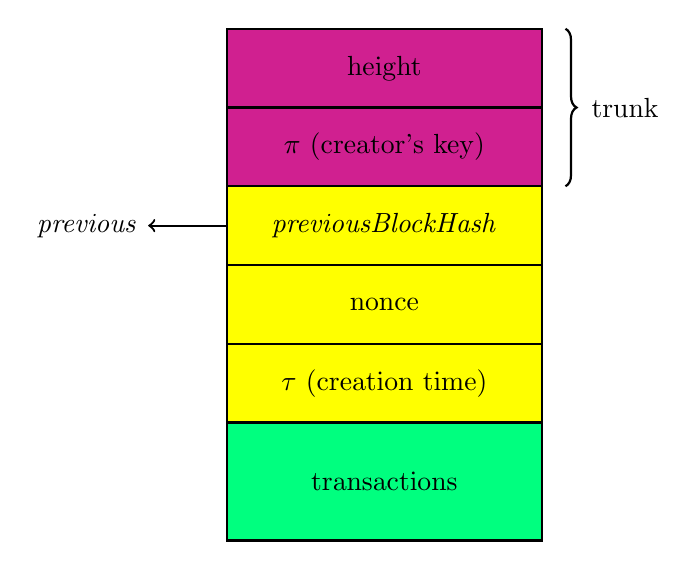
\begin{tikzpicture}
      \draw [decorate,decoration={brace,amplitude=4pt},thick,xshift=0.3cm,yshift=0pt]
      (4,6.5) -- (4,4.5) node [midway,right,xshift=.2cm] {trunk};
      \draw [fill=VioletRed, thick] (0,4.5) rectangle (4,6.5);
      \draw (2,6) node{height};
      \draw [fill=VioletRed, thick] (0,3.5) rectangle (4,5.5);
      \draw (2,5) node{$\pi$ (creator's key)};
      \draw [fill=Yellow, thick] (0,3.5) rectangle (4,4.5);
      \draw (2,4) node{$\previousblockhash$};
      \draw[->,thick] (0,4) -- (-1,4) node [midway,left,xshift=-.5cm] {$\previous$};

      \draw [fill=Yellow, thick] (0,2.5) rectangle (4,3.5);
      \draw (2,3) node{nonce};
      \draw [fill=Yellow, thick] (0,1.5) rectangle (4,2.5);
      \draw (2,2) node{$\tau$ (creation time)};

      \draw [fill=SpringGreen, thick] (0,0) rectangle (4,1.5);
      \draw (2,0.75) node{transactions};
  \end{tikzpicture}
  \end{center}
\end{frame}

\begin{frame}[fragile]{Point~2: Derivation of a challenge from a block}

  \begin{align*}
    \challenge(\genesis)&=\langle 0,\sigma_\genesis\rangle,\quad\sigma_\genesis\text{ is an arbitrary byte array}\\
    \challenge(\block)&=\langle\hash(\sigma\bowtie(\previous.\height+1))\ \mathit{mod}\ n,\sigma\rangle\\
    &\text{where $\sigma=\hash(\challenge(\previous).\sigma\bowtie\pi)$}
  \end{align*}

  \begin{center}
    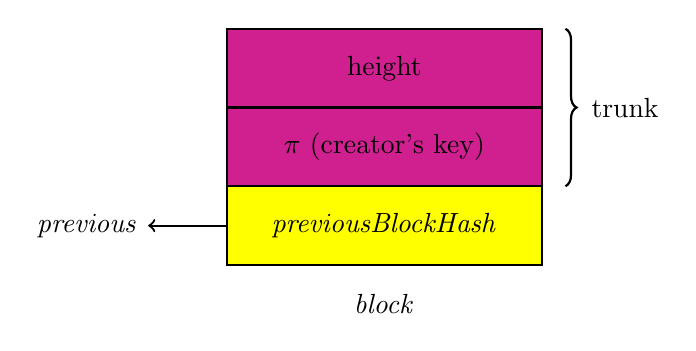
\begin{tikzpicture}
      \draw [decorate,decoration={brace,amplitude=4pt},thick,xshift=0.3cm,yshift=0pt]
      (4,7.5) -- (4,5.5) node [midway,right,xshift=.2cm] {trunk};
      \draw [fill=VioletRed, thick] (0,5.5) rectangle (4,7.5);
      \draw (2,7) node{height};
      \draw [fill=VioletRed, thick] (0,4.5) rectangle (4,6.5);
      \draw (2,6) node{$\pi$ (creator's key)};
      \draw [fill=Yellow, thick] (0,4.5) rectangle (4,5.5);
      \draw (2,5) node{$\previousblockhash$};
      \draw[->,thick] (0,5) -- (-1,5) node [midway,left,xshift=-.5cm] {$\previous$};
      \draw (2,4) node{$\block$};
    \end{tikzpicture}
  \end{center}

  \begin{center}
    \textbf{Proposition.} Challenges depends on the trunks only (simple proof by induction): Signum has no block-grinding attacks
  \end{center}

\end{frame}

\begin{frame}{Point~3: The delay of a nonce \wrt a challenge}

  \begin{center}
  Let $\challenge=\langle i,\sigma\rangle$ and
  $\nonce=\langle p,\underbrace{h_0,h_{2n-1}}_{\scoop_0},\underbrace{h_2,h_{2n-3}}_{\scoop_1},\ldots,\underbrace{h_{2n-4},h_3}_{\scoop_{n-2}},\underbrace{h_{2n-2},h_1}_{\scoop_{n-1}}\rangle$:
  \end{center}
  \bigskip
  \[
    \delay(\nonce,\challenge)=\hash(\scoop_i\bowtie\sigma)
  \]

\end{frame}

\begin{frame}{Miner $\pi'$ selects its best $\nonce'$ and builds a next block}

  \begin{center}
    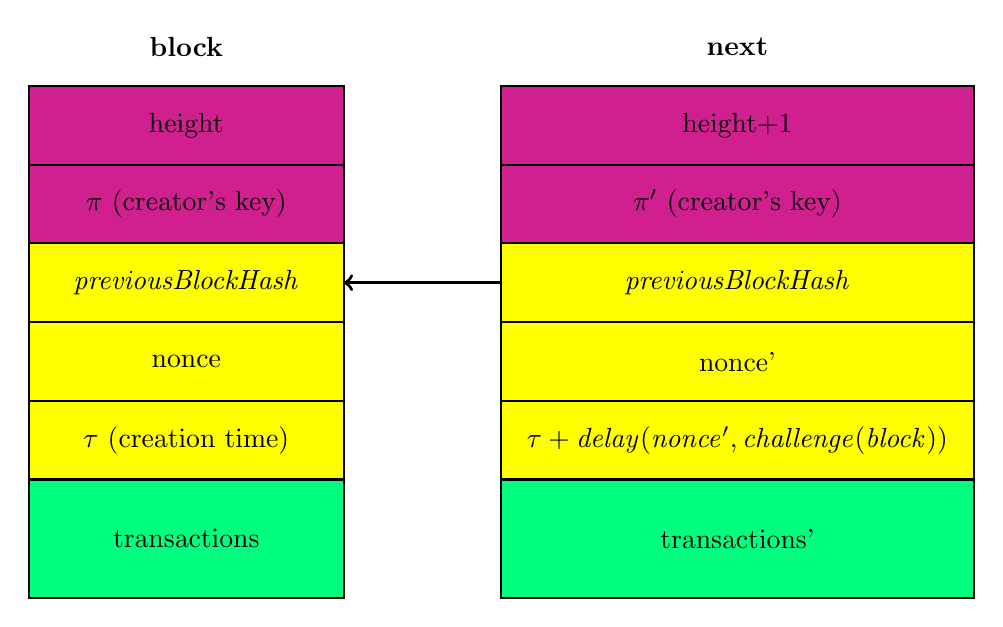
\begin{tikzpicture}
      \draw (2,7) node{\textbf{block}};
      \draw [fill=VioletRed, thick] (0,4.5) rectangle (4,6.5);
      \draw (2,6) node{height};
      \draw [fill=VioletRed, thick] (0,3.5) rectangle (4,5.5);
      \draw (2,5) node{$\pi$ (creator's key)};
      \draw [fill=Yellow, thick] (0,3.5) rectangle (4,4.5);
      \draw (2,4) node{$\previousblockhash$};

      \draw [fill=Yellow, thick] (0,2.5) rectangle (4,3.5);
      \draw (2,3) node{nonce};
      \draw [fill=Yellow, thick] (0,1.5) rectangle (4,2.5);
      \draw (2,2) node{$\tau$ (creation time)};

      \draw [fill=SpringGreen, thick] (0,0) rectangle (4,1.5);
      \draw (2,0.75) node{transactions};

      \visible<2->{
      \draw (9,7) node{\textbf{next}};
      \draw [fill=VioletRed, thick] (6,5.5) rectangle (12,6.5);
      \draw (9,6) node{height+1};
      }
      \visible<3->{
      \draw [fill=VioletRed, thick] (6,4.5) rectangle (12,5.5);
      \draw (9,5) node{$\pi'$ (creator's key)};
      }
      \visible<4->{
      \draw [fill=Yellow, thick] (6,3.5) rectangle (12,4.5);
      \draw (9,4) node{$\previousblockhash$};
      \draw[->,very thick] (6,4) -- (4,4);
      }

      \visible<5->{
      \draw [fill=Yellow, thick] (6,2.5) rectangle (12,3.5);
      \draw (9,3) node{nonce'};
      }
      \visible<6->{
      \draw [fill=Yellow, thick] (6,1.5) rectangle (12,2.5);
      \draw (9,2) node{$\tau+\delay(\nonce',\challenge(\block))$};
      }

      \visible<7->{
      \draw [fill=SpringGreen, thick] (6,0) rectangle (12,1.5);
      \draw (9,0.75) node{transactions'};
      }
    \end{tikzpicture}
  \end{center}

\end{frame}

\begin{frame}\frametitle{Blockchain}

  A \emph{blockchain} is a set $B$ of blocks such that:
  \begin{enumerate}
    \pause
  \item there is exactly one genesis block, written $\genesis(B)$
    \pause
  \item for each hash $h$, there is at most a $\block\in B$ s.t.\ $\hash(\block)=h$,
    written $\block(B,h)$
    \pause
  \item every $\block\in B$ satisfies the consensus rules:
    \begin{enumerate}
      \pause
    \item[a] no block is created in the future: $\block.\tau\le\tau_\now$
      \pause
    \item[] Moreover, if $\block\not=\genesis(B)$:
      \pause
    \item[b] no dangling pointers: $\previous=\block(B,\block.\previousblockhash)$ exists
%    \item[c] the deadline $\delta=b.\trunk.\delta$ of $b$ is valid
%    \item[d] $\delta$ answers the challenge of $p$:
      %      $\challenge_\mynext(p)=\delta.\challenge$
      \pause
    \item[c] height increases: $\block.\height=\previous.\height+1$
      \pause
    \item[d] the delay of the nonce has expired: $\block.\tau=\previous.\tau+\delay(\block.\nonce,\challenge(\previous))$
      \pause
    \item[e] the nonce is for the creator of the block:
      $\block.\nonce=\nonce(\block.\nonce.p,\block.\pi)$
    \end{enumerate}
  \end{enumerate}
\end{frame}

\begin{frame}{The life of a blockchain peer}

  A blockchain peer computer holds:
  \begin{itemize}
  \item a blockchain $B$
  \item a set of nonces precomputed on disk, called $\plot$
  \item a network connection to some other peers
  \end{itemize}

  \bigskip
  \pause
  It performs two algorithms concurrently:
  \begin{enumerate}
    \pause
  \item the block mining algorithm (produce blocks and send them to peers)
    \pause
  \item the block mined algorithm (receive blocks from peers and check them)
  \end{enumerate}

\end{frame}

\begin{frame}{The block mining algorithm}

  \begin{greenbox}{An infinite loop}
    \begin{enumerate}[<+->]
    \item\label{step:block_mining:loop} identify a most powerful $\mathbf{block}\in B$
    \item\label{step:block_mining:next_challenge} compute $c=\challenge(\mathbf{block})$
    \item\label{step:block_mining:next_deadline} identify a nonce $\nu$ in $\plot$ that minimizes $\delay(\nu,c)$
    \item\label{step:block_mining:next_block} build block \textbf{next} by using $\nu$
    \item\label{step:block_mining:wait} wait until $\mathbf{next}.\tau\le\tau_\now$
    \item\label{step:block_mining:add} add $\mathbf{next}$ to $B$ [no check: consensus holds for $\mynext$ by construction]
    \item\label{step:block_mining:whisper} whisper $\mathbf{next}$ to the connected peers
    \item go back to step~\ref{step:block_mining:loop}
    \end{enumerate}
  \end{greenbox}

\end{frame}

\begin{frame}{The block mined algorithm}

  \begin{greenbox}{An infinite loop}
    \begin{enumerate}[<+->]
    \item\label{step:block_mined:loop} wait for a \textbf{block} whispered from some connected peer $P'$
    \item\label{step:block_mined:add} if $B\cup\{\mathbf{block}\}$ is a blockchain, add $\mathbf{block}$ to $B$ [consensus check: peers might be cheating]
    \item go back to step~\ref{step:block_mined:loop}
    \end{enumerate}
  \end{greenbox}

\end{frame}

\begin{frame}{Challenge-grinding attacks are complicated and expensive}

  \begin{center}
    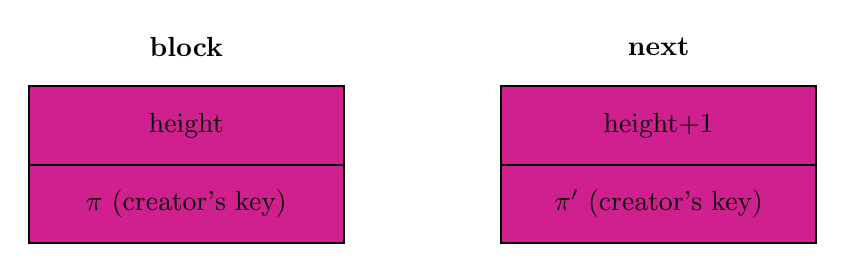
\begin{tikzpicture}
      \draw (2,7) node{\textbf{block}};
      \draw [fill=VioletRed, thick] (0,5.5) rectangle (4,6.5);
      \draw (2,6) node{height};
      \draw [fill=VioletRed, thick] (0,4.5) rectangle (4,5.5);
      \draw (2,5) node{$\pi$ (creator's key)};

      \draw (8,7) node{\textbf{next}};
      \draw [fill=VioletRed, thick] (6,5.5) rectangle (10,6.5);
      \draw (8,6) node{height+1};

      \draw [fill=VioletRed, thick] (6,4.5) rectangle (10,5.5);
      \draw (8,5) node{$\pi'$ (creator's key)};
    \end{tikzpicture}
  \end{center}

  Challenge-grinding attacks are only possible if a miner grinds over many impersonations $\pi'$, but:

  \begin{enumerate}
    \pause
  \item this requires to recompute nonces on-the-fly for each impersonation: very expensive
    \pause
  \item this requires to recollect mining fees from all used impersonations: complicated
    and expensive (transfer fees)
  \end{enumerate}

  \pause
  \begin{center}
    \textbf{Proposition.} Signum is largely protected from challenge-grinding attacks.
  \end{center}

\end{frame}

\begin{frame}\frametitle{Protection against newborn attacks}

  \begin{redbox}{Problem: the same plot file can be used for mining for many distinct blockchain
      networks using the Signum protocol}
    Who has allocated a big plot file for an established network can use it for free
    for mining \textbf{(concurrently!)} for another, newborn, small network and effectively take its control!
  \end{redbox}

  \medskip

  Expensive with PoW: CPU power can only be used for a single network

  \bigskip

  \visible<2->{
  \begin{greenbox}{Solution}
    Enrich $\pi$ with extra information about:
    \begin{itemize}
    \item chain name
    \item chain id
    \item genesis time
    \item \ldots
    \end{itemize}
    Add a consensus rule that checks such extra data
  \end{greenbox}
  }

\end{frame}

\begin{frame}\frametitle{Protection against censorship attacks}

  \begin{center}
    \begin{tikzpicture}
      \draw [decorate,decoration={brace,amplitude=4pt},thick,xshift=0.3cm,yshift=0pt]
      (6,6.5) -- (6,4.5) node [midway,right,xshift=.2cm] {trunk};
      \draw [fill=VioletRed, thick] (0,4.5) rectangle (6,6.5);
      \draw (3,6) node{height};
      \draw [fill=VioletRed, thick] (0,3.5) rectangle (6,5.5);
      \draw (3,5) node{$\pi$ (creator's key)};
      \draw [fill=Yellow, thick] (0,3.5) rectangle (6,4.5);
      \draw (3,4) node{$\previousblockhash$};
      \draw[->,thick] (0,4) -- (-1,4) node [midway,left,xshift=-.5cm] {$\previous$};

      \draw [fill=Yellow, thick] (0,2.5) rectangle (6,3.5);
      \draw (3,3) node{nonce};
      \draw [fill=Yellow, thick] (0,1.5) rectangle (6,2.5);
      \draw (3,2) node{$\tau$ (creation time)};

      \draw [fill=SpringGreen, thick] (0,0.5) rectangle (6,1.5);
      \only<1,3>{\draw (3,1) node{\textbf{\Large $\Rightarrow$transactions$\Leftarrow$}};}
      \only<2>{\draw (3,1) node{\textbf{\Large $\Rightarrow$censored transactions$\Leftarrow$}};}

      \visible<3>{
      \draw [fill=SkyBlue, thick] (0,-0.5) rectangle (6,0.5);
      \draw (3,0) node{$\pi$'s signature};
      }

    \end{tikzpicture}
  \end{center}

  \begin{center}
    \only<1>{Transactions are not used for mining}
    \only<2>{Transactions can be replaced with any set of censored transactions!}
    \only<3>{Solution: sign with $\pi$'s private key and add a consensus rule to check it}
  \end{center}

\end{frame}

\begin{frame}{Optimization: deadlines instead of nonces}

  \begin{center}
    \begin{tikzpicture}
      \draw [decorate,decoration={brace,amplitude=4pt},thick,xshift=0.3cm,yshift=0pt]
      (4,6.5) -- (4,4.5) node [midway,right,xshift=.2cm] {trunk};
      \draw [fill=VioletRed, thick] (0,4.5) rectangle (4,6.5);
      \draw (2,6) node{height};
      \draw [fill=VioletRed, thick] (0,3.5) rectangle (4,5.5);
      \draw (2,5) node{$\pi$ (creator's key)};
      \draw [fill=Yellow, thick] (0,3.5) rectangle (4,4.5);
      \draw (2,4) node{$\previousblockhash$};
      \draw[->,thick] (0,4) -- (-1,4) node [midway,left,xshift=-.5cm] {$\previous$};

      \draw [fill=Yellow, thick] (0,2.5) rectangle (4,3.5);
      \only<1>{\draw (2,3) node{\textbf{\Large $\Rightarrow$nonce$\Leftarrow$}};}
      \only<2>{\draw (2,3) node{\textbf{\Large $\Rightarrow$deadline$\Leftarrow$}};}
      \draw [fill=Yellow, thick] (0,1.5) rectangle (4,2.5);
      \draw (2,2) node{$\tau$ (creation time)};

      \draw [fill=SpringGreen, thick] (0,0.5) rectangle (4,1.5);
      \draw (2,1) node{transactions};
      \draw [fill=SkyBlue, thick] (0,-0.5) rectangle (4,0.5);
      \draw (2,0) node{$\pi$'s signature};
    \end{tikzpicture}
  \end{center}

  \begin{center}
    \only<1>{A nonce is too big for each block ($262$ Kbytes)}
    \only<2>{Replace it with a compact representation called deadline ($200$ bytes)}
  \end{center}

\end{frame}

\begin{frame}\frametitle{Conclusion}

  The only existing formalization of Signum:

  \begin{itemize}
  \item it clarifies how Signum works
  \item it proves that the suspected block-grinding attack cannot occur
  \item it proves that the suspected time-memory trade-off does not exist (but others might exist! a general proof is still missing)
  \item it proves that challenge-grinding attacks are impractical
  \item it introduces a new protection against newborn attacks
  \end{itemize}

\end{frame}

\end{document}
